\section{Getting Started C}

In this tutorial you will get a first look at a very simple \eTrice{} model. The goal is to learn the work flow of \eTrice{} and to understand a few basic features of ROOM.

\textbf{Preconditions}:
\begin{itemize}
	\item Working C development environment with CDT Eclipse
	\begin{itemize}
		\item C compiler: MinGW/GCC (Windows) or Posix/GCC (Linux)
		\item Installed C/C++ Development Tools (CDT) in Eclipse
	\end{itemize}
	\item Activated \emph{Build Automatically} option in Eclipse: \emph{Project -> Build Automatically}
	\item Recommended: Activate automatic resource refresh in Eclipse: \emph{Window -> Preferences -> General -> Workspace}
	\begin{itemize}
		\item \emph{Refresh using native hooks or polling}
		\item \emph{Refresh on access}
	\end{itemize}
	\item Optional: Install \href{http://trace2uml.stage.tigris.org/}{Trace2UML}, a Open Source MSC viewer
	\begin{itemize}
		\item \href{http://trace2uml.tigris.org/servlets/ProjectDocumentList?folderID=6208}{Windows download site}
		\item \href{http://apt.astade.de/}{Linux package}
	\end{itemize}

\end{itemize}

\subsection{Create template project}
After installation of \eTrice in Eclipse, we can use the wizard to create the \emph{template.c} project, which is good starting point for new ROOM applications. Select the menu \emph{File -> New -> Other} (Ctrl+N) and choose \emph{eTrice C Template Project}. To complete the wizard press \emph{Next} and on the next page \emph{Finish}.

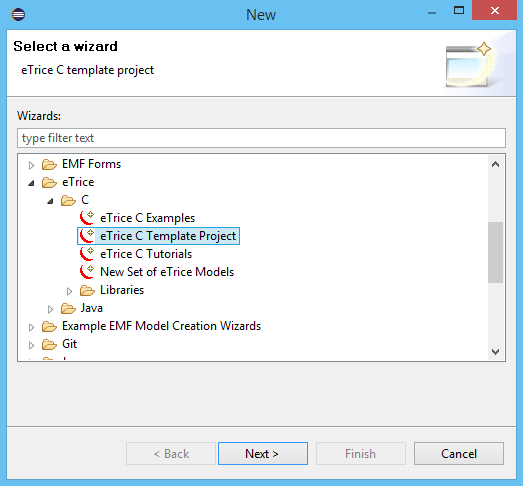
\includegraphics[width=.5\textwidth]{images/013-wizard.png}

This will add three projects into your workspace, the library projects \emph{runtime.c} and \emph{modellib.c} and our application project \emph{template.c}. Now open the \emph{TemplateModel.room} in the model folder of \emph{template.c}.

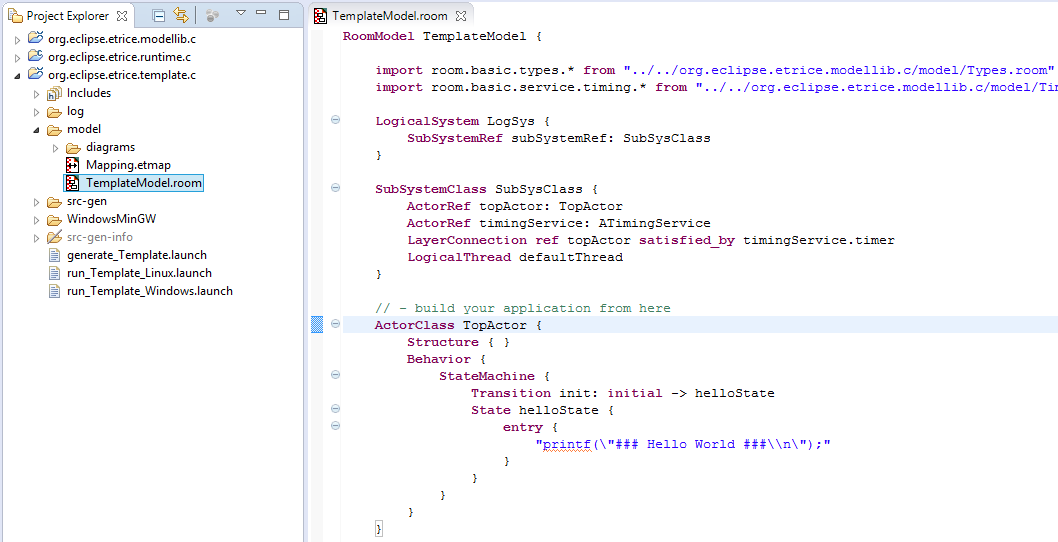
\includegraphics[width=\textwidth]{images/013-after-wizard.png}

The model contains an ActorClass \emph{TopActor}, which is currently the only active actor. TopActor has a state machine that is intended to output a simple HelloWorld statement. To inspect its behavior graphically, we can open the behavior diagram by right click on \emph{Outline View -> TopActor -> Edit Behavior}. Alternatively we can place the cursor within the textual notation and press Alt+B.

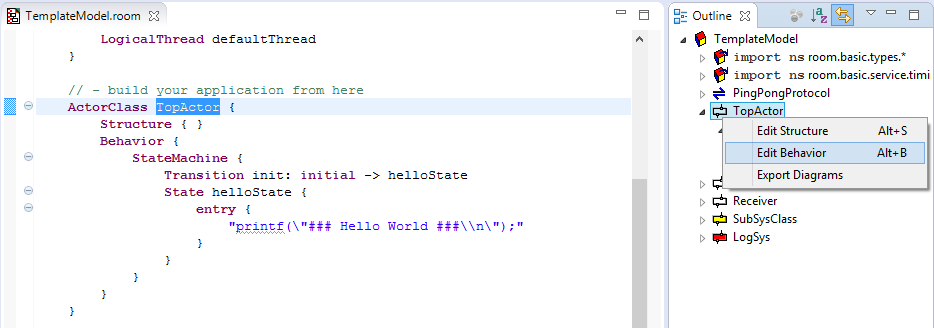
\includegraphics[width=\textwidth]{images/013-open-hello-fsm.png}

The state machine has an initial transition that leads to \emph{helloState}. The state defines an entry code, which is executed during the transition. We can view the details by hovering over the state and edit the code with a double-click or right click and \emph{Edit State}.

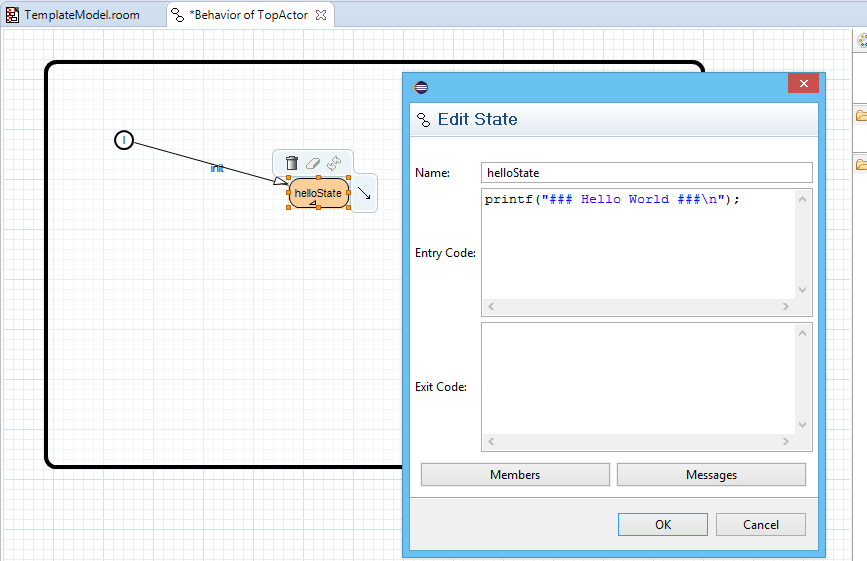
\includegraphics[width=\textwidth]{images/013-hello-fsm.png}

\subsection{Generate and run application}

Now we are ready to translate the model into an executable application. The first step is to generate source files from the model. Therefore we run the eTrice model generator by right click on file \begin{quote}
	\emph{generate\_Template.launch -> Run As -> generate\_Template}.
\end{quote}
After that we can build and run the application by right click on file
\begin{quote}
	 \emph{run\_Template\_Windows.launch -> Run As -> run\_Template\_Windows}
\end{quote}.
This will trigger the build process, carried out by CDT Eclipse and then subsequently start our application.

\begin{tabular}{cc}
	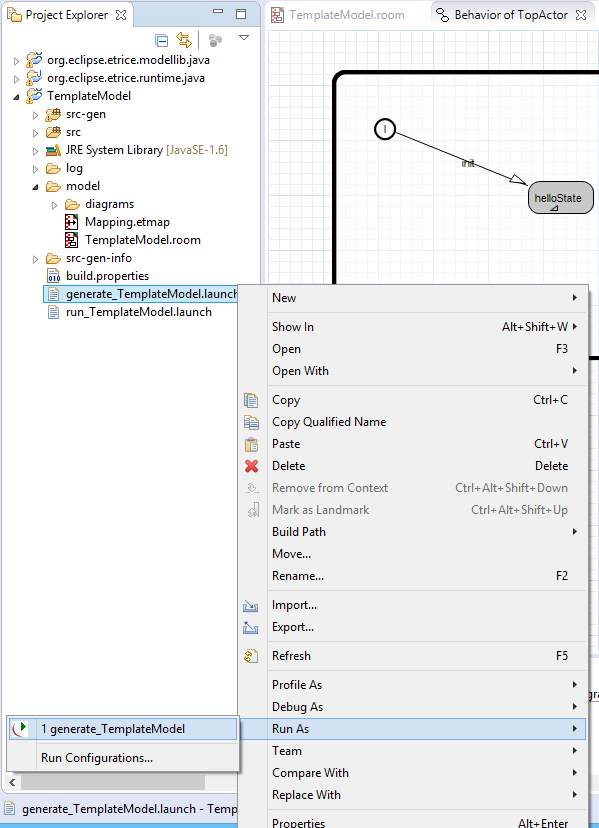
\includegraphics[width=.45\textwidth]{images/014-generate.png} & 
	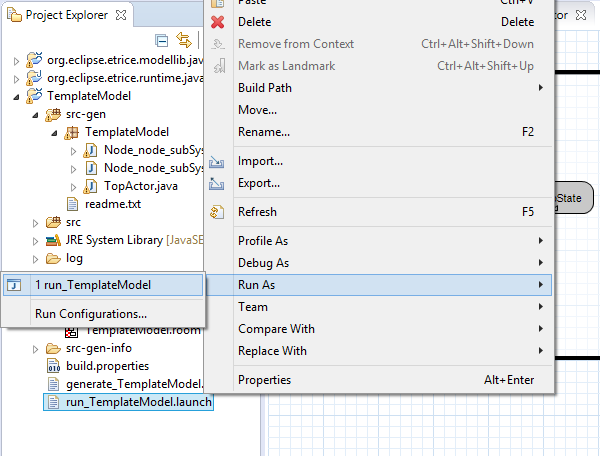
\includegraphics[width=.45\textwidth]{images/014-build_run.png} \\
	1. Invoke generator & 2. Build and run application
\end{tabular}

The output of our application is logged in the Console View and it shows the "Hello World". By typing "quit", as prompt, and pressing enter, the application terminates regularly.

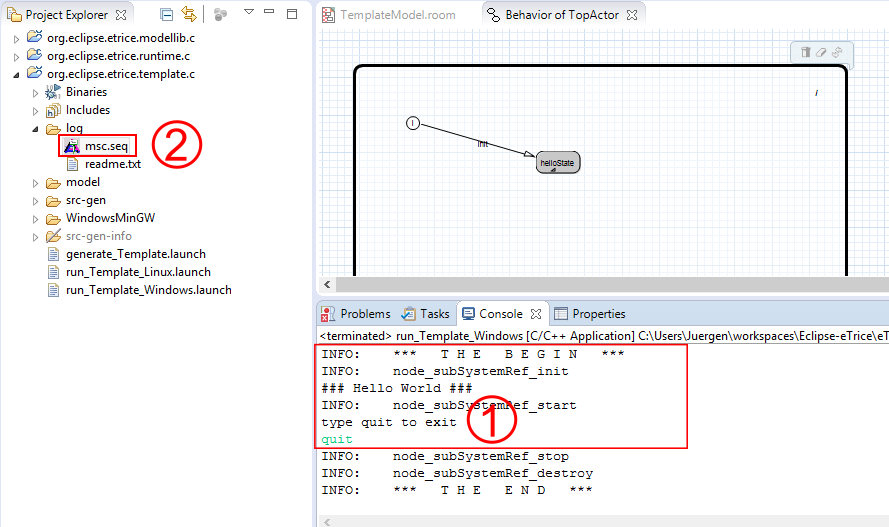
\includegraphics[width=\textwidth]{images/013-quit-hello-msc.png}

\subsection{Open the Message Sequence Chart}

For debugging and learning purposes, the application produced a Message Sequence Chart and wrote it to a file. Open the file \emph{subSysRef1\_Async.seq} or \emph{msc.seq} in the folder \emph{HelloWorld/tmp/log/} using the tool Trace2UML. Create the path if not already there.

Trace2UML is an open source MSC viewer and can be obtained here:
\begin{itemize}
\item \href{http://trace2uml.tigris.org/}{Trace2UML project home and download of windows version} 
\item \href{http://apt.astade.de/}{download of the Linux package of the Astade UML tool which contains Trace2UML}
\end{itemize}
After opening the file, you should see something like this:

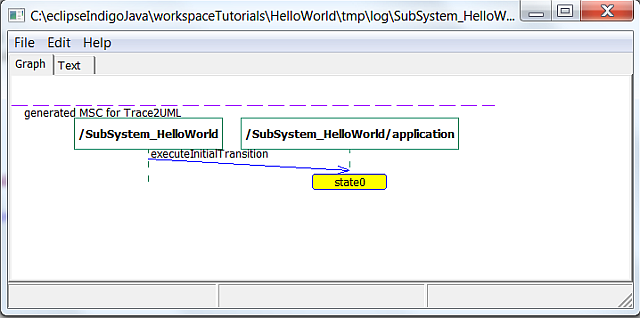
\includegraphics[width=0.6\textwidth]{images/015-HelloWorld09.png}
% !images/015-HelloWorld09.png!

The Actor with the instance path \emph{/LogSys1/subSysRef1/actorRef1} is in the state \emph{state0}. 
This is the simplest possible MSC. The MSCs for further tutorials will contain more information.

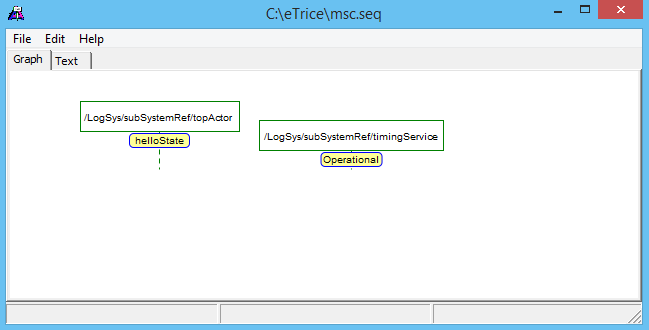
\includegraphics[width=0.6\textwidth]{images/013-hello-msc.png}
